\section{(Dreh-)Streckungen}\label{kapitel:Drehstreckungen}
Seid ihr gut darin, in einer Skizze ähnliche Dreiecke zu erraten? Der Autor dieses Kapitels definitiv nicht! Wenn euch das genauso geht, dann ist dieses Kapitel genau richtig für euch. Drehstreckungen sind ein sehr nützliches Hilfsmittel, um über geometrische Konfigurationen nachzudenken. Wenn ihr diese Denkweise einmal verinnerlicht habt, wird es euch leichter fallen, ähnliche Dreiecke, kollineare Punkte und andere Beziehungen zu erkennen.

\subsection*{Allgemeine Theorie}
\begin{definition}
	Eine \emph{orientierungserhaltende Ähnlichkeitsabbildung} ist eine Abbildung der Euklidischen Ebene auf sich selber, sodass für beliebige drei Punkte $A$,~$B$,~$C$ und ihre Bildpunkte $A'$,~$B'$,~$C'$ die Dreiecke $ABC$ und $A'B'C'$ gleichsinnig ähnlich sind.
\end{definition}

Orientierungserhaltende Ähnlichkeitsabbildungen können folgendermaßen klassifiziert werden:

\begin{satzmitnamen}[Klassifikation von orientierungserhaltenden Ähnlichkeitsabbildungen]
	Jede orientierungserhaltende Ähnlichkeitsabbildung ist eine Drehstreckung oder eine Verschiebung. Ferner gilt:
	\begin{enumerate}
		\item \label{itm:Drehstreckung}
		Die Hintereinanderausführung von zwei Drehstreckungen \embrace{die nicht notwendigerweise das gleiche Zentrum haben müssen} ist wieder eine Drehstreckung oder eine Verschiebung.
		\item \label{itm:Streckung}
		Die Hintereinanderausführung von zwei Streckungen \embrace{die nicht notwendigerweise das gleiche Zentrum haben müssen} ist wieder eine Streckung oder eine Verschiebung.
		\item \label{itm:Drehung}
		Die Hintereinanderausführung von zwei Drehungen \embrace{die nicht notwendigerweise das gleiche Zentrum haben müssen} ist wieder eine Drehung oder eine Verschiebung.
	\end{enumerate}
\end{satzmitnamen}

Zum Beweis benutzen wir ein Lemma, das auch für sich genommen nützlich sein kann.

\begin{satzmitnamen}[Lemma]
	Seien $\omega_1$~und~$\omega_2$ zwei Kreise, die sich in $P$~und~$Q$ schneiden. Sei $\sigma$ die Drehstreckung mit Zentrum~$P$, die $\omega_1$ auf~$\omega_2$ abbildet. Dann ist $\sigma$ identisch mit der Projektion durch~$Q$. Das bedeutet: Für jeden Punkt~$X$ auf~$\omega_1$ ist $\sigma(X)$ der zweite Schnittpunkt von~$XQ$ mit~$\omega_2$ \embrace{im Fall $X=Q$ interpretieren wir $XQ$ als die Tangente an~$\omega_1$ in~$Q$}.
\end{satzmitnamen}

\begin{figure}[ht]
	\centering
	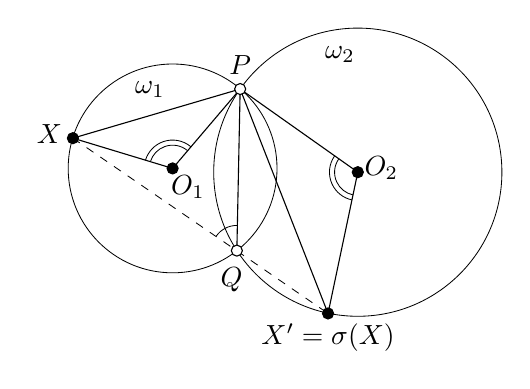
\begin{tikzpicture}[x=0.6cm,y=0.6cm]
		\coordinate (O1) at (-1.54,2.1);
		\coordinate (O2) at (2.38,2.02);
		\coordinate (P) at (-0.11,3.78);
		\coordinate (Q) at (-0.18,0.36);
		\coordinate (X) at (-3.65,2.74);
		\coordinate (X1) at (1.75,-0.97);
		\draw [shift={(-0.18,0.36)}, line width=0.3] (88.83:0.32cm) arc (88.83:145.53:0.32cm);
		\draw (Q) to (P) to (X) to (O1) to (P) to (O2) to (X1) to (P);
		\draw [line width=0.3] (-1.54,2.1) circle (2.21);
		\draw [line width=0.3] (2.38,2.02) circle (3.05);
		\draw[dashed, line width=0.3]  (X) to (X1);
		\draw [shift={(-1.54,2.1)}, line width=0.3] (49.65:0.6) arc (49.65:163.05:0.6);
		\draw [shift={(-1.54,2.1)}, line width=0.3] (49.65:0.491667) arc (49.65:163.05:0.491667);
		\draw [shift={(2.38,2.02)}, line width=0.3] (144.70:0.6) arc (144.70:258.10:0.6);
		\draw [shift={(2.38,2.02)}, line width=0.3] (144.70:0.491667) arc (144.70:258.10:0.491667);
		\draw [fill=black] (O1) circle (2pt) node[shift={(310:2ex)}] {$O_1$};
		\draw [fill=white] (Q) circle (2pt) node[shift={(260:2.5ex)}] {$Q$};
		\draw [fill=black] (O2) circle (2pt) node[shift={(10:2ex)}] {$O_2$};
		\draw [fill=white] (P) circle (2pt) node[shift={(90:2ex)}] {$P$};
		\draw [fill=black] (X) circle (2pt) node[shift={(170:2ex)}] {$X$};
		\draw [fill=black] (X1) circle (2pt) node[shift={(270:2ex)}] {$X'=\sigma(X)$};
		\node at (-2.02,3.77) {$\omega_1$};
		\node at (2,4.51) {$\omega_2$};
	\end{tikzpicture}
\end{figure}

\begin{proof}
	Wir betrachten nur den Fall, dass $X$ auf dem Kreisbogen~$\wideparen{PQ}$ von~$\omega_1$ liegt, der außerhalb von~$\omega_2$ verläuft; der andere Fall geht analog. Sei $X'$ der zweite Schnittpunkt von~$XQ$ mit~$\omega_2$ und seien $O_1$,~$O_2$ die Mittelpunkte von $\omega_1$,~$\omega_2$. Die Drehstreckung~$\sigma$ bildet $O_1$ auf~$O_2$ ab und $P$~auf sich selbst. Es genügt also, $\winkel PO_1X=\winkel PO_2X'$ zu zeigen. Nach dem Zentri-Peripheriewinkelsatz gilt nun $\winkel PO_1X=2\winkel PQX$ und $\winkel X'O_2P=2\winkel X'QP$. Also ist
	\begin{equation*}
		\winkel PO_2X'=360^\circ-\winkel X'O_2P=2(180^\circ-\winkel X'QP)=2\winkel PQX=\winkel PO_1X,
	\end{equation*}
	wie gewünscht.
\end{proof}

\begin{proof}[Beweis der Klassifikation]
	Offensichtlich sind Drehstreckungen und Verschiebungen orientierungserhaltende Ähnlichkeitsabbildungen. Sei umgekehrt $\sigma$ eine orientierungserhaltende Ähnlichkeitsabbildung. Wähle zwei verschiedene Punkte $A$~und~$B$ sowie ihre Bildpunkte $A'\coloneqq \sigma(A)$ und $B'\coloneqq \sigma(B)$. Für jeden weiteren Punkt~$X$ ist der Bildpunkt $X'\coloneqq\sigma(X)$ eindeutig dadurch bestimmt, dass die Dreiecke $ABX$ und $A'B'X'$ gleichsinning ähnlich sein müssen. Es genügt also zu zeigen, dass stets eine Drehstreckung oder eine Verschiebung~$\sigma'$ existiert, die $A$~auf~$A'$ und $B$~auf~$B'$ abbildet. Denn aus der eben festgestellten Eindeutigkeit folgt dann auch $\sigma(X)=\sigma'(X)$ für jeden weiteren Punkt~$X$, sodass zwangsläufig $\sigma=\sigma'$ ist.
	
	Um $\sigma'$ zu konstruieren, unterscheiden wir (in aufsteigender Allgemeinheit) drei Fälle:
	\begin{figure}[ht]
		\centering
		\begin{tabularx}{\textwidth}{X c X c X c X}
			& 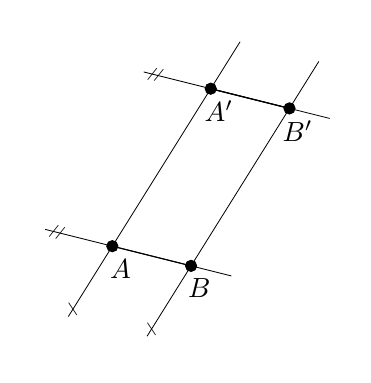
\begin{tikzpicture}[x=0.5cm,y=0.5cm]
				\clip (-2.15,-2.75) rectangle (5.85,5.55);
				\coordinate (A) at (0,0);
				\coordinate (B) at (2,-0.5);
				\coordinate[shift={(2.5,4)}] (A1) at (A);
				\coordinate[shift={(2.5,4)}] (B1) at (B);
				\draw (A) to (B);
				\draw (A1) to (B1);
				\draw[line width=0.3, shorten <=-2.5em,shorten >=-1.5em] (A) to node[pos=-0.7,sloped] {$\scriptscriptstyle/\!/$} (B);
				\draw[line width=0.3, shorten <=-2.5em,shorten >=-1.5em] (A1) to node[pos=-0.7,sloped] {$\scriptscriptstyle/\!/$} (B1);
				\draw[line width=0.3, shorten <=-3em,shorten >=-2em] (A) to node[pos=-0.4,sloped] {$\scriptscriptstyle/$} (A1);
				\draw[line width=0.3, shorten <=-3em,shorten >=-2em] (B) to node[pos=-0.4,sloped] {$\scriptscriptstyle/$} (B1);
				\draw (A1) to (B1);
				%\draw [transform canvas={shift={(4.5,-1.125)}},->] (A) to node[shift={(150:2ex)}] {$\sigma'$} (A1);
				\draw [fill=black] (A) circle (2pt) node[shift={(290:2ex)}] {$A$};
				\draw [fill=black] (B) circle (2pt) node[shift={(290:2ex)}] {$B$};
				\draw [fill=black] (A1) circle (2pt) node[shift={(290:2ex)}] {$A'$};
				\draw [fill=black] (B1) circle (2pt) node[shift={(290:2ex)}] {$B'$};
			\end{tikzpicture} & & 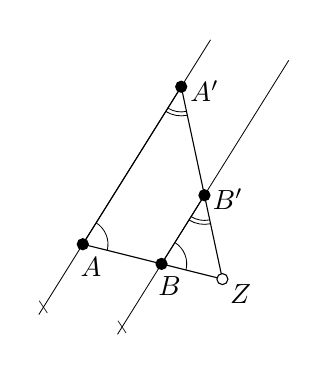
\begin{tikzpicture}[x=0.5cm,y=0.5cm]
				\clip (-1.4,-2.72) rectangle (5.7,5.5);
				\coordinate (A) at (0,0);
				\coordinate (B) at (2,-0.5);
				\coordinate (A1) at (2.5,4);
				\coordinate (B1) at (3.09,1.244);
				\coordinate (Z) at (3.546,-0.886);
				\draw (B1) to (A1) to (A) to (Z) to (B1) to (B);
				\draw[line width=0.3, shorten <=-3em,shorten >=-2em] (A) to node[pos=-0.4,sloped] {$\scriptscriptstyle/$} (A1);
				\draw[line width=0.3, shorten <=-3em,shorten >=-5.75em] (B) to node[pos=-0.92,sloped] {$\scriptscriptstyle/$} (B1);
				\draw [line width=0.3, shift={(B)}] (-14.036:0.32cm) arc (-14.036:57.995:0.32cm);
				\draw [line width=0.3, shift={(A)}] (-14.036:0.32cm) arc (-14.036:57.995:0.32cm);
				\draw [line width=0.3, shift={(B1)}] (237.995:0.32cm) arc (237.995:282.082:0.32cm);
				\draw [line width=0.3, shift={(B1)}] (237.995:0.37cm) arc (237.995:282.082:0.37cm);
				\draw [line width=0.3, shift={(A1)}] (237.995:0.32cm) arc (237.995:282.082:0.32cm);
				\draw [line width=0.3, shift={(A1)}] (237.995:0.37cm) arc (237.995:282.082:0.37cm);
				\draw [fill=black] (A) circle (2pt) node[shift={(290:2ex)}] {$A$};
				\draw [fill=black] (B) circle (2pt) node[shift={(290:2ex)}] {$B$};
				\draw [fill=black] (A1) circle (2pt) node[shift={(-10:2ex)}] {$A'$};
				\draw [fill=black] (B1) circle (2pt) node[shift={(-10:2ex)}] {$B'$};
				\draw [fill=white] (Z) circle (2pt) node[shift={(320:2ex)}] {$Z$};
			\end{tikzpicture} & & 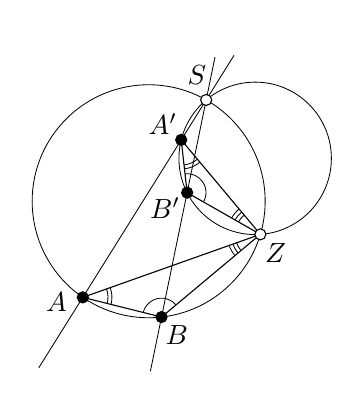
\begin{tikzpicture}[x=0.5cm,y=0.5cm]
				\clip (-1.4,-2.25) rectangle (6.4,6.85);
				\draw [line width=0.3] (1.673,2.441) circle (2.959);
				\draw [line width=0.3] (4.378,3.531) circle (1.936);
				\coordinate (A) at (0,0);
				\coordinate (B) at (2,-0.5);
				\coordinate (A1) at (2.5,4);
				\coordinate (B1) at (2.65,2.66);
				\coordinate (S) at (3.134,5.014);
				\coordinate (Z) at (4.51,1.6);
				\draw (Z) to (A) to (B) to (Z) to (A1) to (B1) to (Z);
				\draw[line width=0.3, shorten <=-3em,shorten >=-3.6em] (A) to (A1);
				\draw[line width=0.3, shorten <=-2em,shorten >=-5em] (B) to (B1);
				\draw [line width=0.3, shift={(A)}] (-14.036:0.32cm) arc (-14.036:19.532:0.32cm);
				\draw [line width=0.3, shift={(A)}] (-14.036:0.37cm) arc (-14.036:19.532:0.37cm);
				\draw [line width=0.3, shift={(B)}] (39.918:0.24cm) arc (39.918:165.964:0.24cm);
				\draw [line width=0.3, shift={(Z)}] (199.532:0.32cm) arc (199.532:219.918:0.32cm);
				\draw [line width=0.3, shift={(Z)}] (199.532:0.37cm) arc (199.532:219.918:0.37cm);
				\draw [line width=0.3, shift={(Z)}] (199.532:0.42cm) arc (199.532:219.918:0.42cm);
				\draw [line width=0.3, shift={(A1)}] (276.374:0.32cm) arc (276.374:309.942:0.32cm);
				\draw [line width=0.3, shift={(A1)}] (276.374:0.37cm) arc (276.374:309.942:0.37cm);
				\draw [line width=0.3, shift={(B1)}] (-29.672:0.24cm) arc (-29.672:96.374:0.24cm);
				\draw [line width=0.3, shift={(Z)}] (129.942:0.32cm) arc (129.942:150.328:0.32cm);
				\draw [line width=0.3, shift={(Z)}] (129.942:0.37cm) arc (129.942:150.328:0.37cm);
				\draw [line width=0.3, shift={(Z)}] (129.942:0.42cm) arc (129.942:150.328:0.42cm);
				\draw [fill=black] (A) circle (2pt) node[shift={(190:2.25ex)}] {$A$};
				\draw [fill=black] (B) circle (2pt) node[shift={(310:2ex)}] {$B$};
				\draw [fill=black] (A1) circle (2pt) node[shift={(140:2ex)}] {$A'$};
				\draw [fill=black] (B1) circle (2pt) node[shift={(215:2.25ex)}] {$B'$};
				\draw [fill=white] (Z) circle (2pt) node[shift={(310:2ex)}] {$Z$};
				\draw [fill=white] (S) circle (2pt) node[shift={(110:2.25ex)}] {$S$};
			\end{tikzpicture} & \\\addlinespace
			& Fall~1 & & Fall~2 & & Fall~3 & 
		\end{tabularx}
	\end{figure}
	
	\emph{Fall~1: Es gilt $AA'\parallel BB'$ und $AB\parallel A'B'$.}
	In diesem Fall ist $ABB'A'$ ein Parallelogramm und wir können $\sigma'$ als diejenige Verschiebung wählen, die $\overline{AB}$ auf~$\overline{A'B'}$ abbildet.
	
	\emph{Fall~2: Es gilt $AA'\parallel BB'$, aber $AB\nparallel A'B'$.}
	In diesem Fall sei $Z$ der Schnittpunkt von $AB$ und~$A'B'$. Sei $\sigma'$ die Drehstreckung mit Zentrum~$Z$, die $A$~auf~$A'$ abbildet. Nach dem Strahlensatz sind die Dreiecke $AA'Z$ und $BB'Z$ gleichsinnig ähnlich, weshalb $\sigma'$ auch $B$~auf~$B'$ abbildet.
	
	\emph{Fall~3: Es gilt $AA'\nparallel BB'$.}
	Sei $S$ der Schnittpunkt von $AA'$~und~$BB'$ und sei $Z$ der zweite Schnittpunkt der Umkreise $\odot ABS$ und $\odot A'B'S$ (falls sich die Umkreise in~$S$ tangieren, wählen wir $Z=S$). Sei $\sigma'$ die Drehstreckung mit Zentrum~$Z$, die Kreis $\odot ABSZ$ auf den Kreis $\odot A'B'SZ$ abbildet. Aus dem Lemma folgt dann direkt, dass $\sigma'$ den Punkt $A$ auf $A'$ und den Punkt $B$ auf $B'$ abbildet, wie gewünscht.
	
	Damit ist gezeigt, dass jede orientierungserhaltende Ähnlichkeitsabbildung eine Drehstreckung oder eine Verschiebung ist. Die weiteren Behauptungen \ref{itm:Drehstreckung}~und~\ref{itm:Streckung} sind nun einfache Folgerungen: Wenn $\sigma_1$~und~$\sigma_2$ Drehstreckungen sind, dann ist die Hintereinanderausführung $\sigma_2\circ \sigma_1$ offensichtlich wieder eine orientierungserhaltende Ähnlichkeitsabbildung, also eine Drehstreckung oder eine Verschiebung. Damit ist Behauptung~\ref{itm:Drehstreckung} gezeigt.
	
	Für Behauptung~\ref{itm:Streckung} betrachte den Fall, dass $\sigma_1$~und~$\sigma_2$ Streckungen sind. Wir wissen schon, dass $\sigma_2\circ \sigma_1$ eine Drehstreckung oder eine Verschiebung sein muss. Wenn wir eine Verschiebung vorliegen haben, sind wir fertig. Wir nehmen also an, dass $\sigma_2\circ \sigma_1$ eine Drehstreckung ist. Streckungen schicken aber Geraden auf parallele Geraden. Für jede Gerade $\ell$ ist demzufolge  $\ell\parallel\sigma_1(\ell)\parallel \sigma_2(\sigma_1(\ell))$. Der Drehwinkel von $\sigma_2\circ \sigma_1$ muss also $0^\circ$~oder~$180^\circ$ sein und somit haben wir es in der Tat mit einer Streckung (möglicherweise mit negativem Streckfaktor) zu tun.
	
	Für Behauptung~\ref{itm:Drehung} betrachte den Fall, dass $\sigma_1$~und~$\sigma_2$ Streckungen sind. Wir wissen schon, dass $\sigma_2\circ \sigma_1$ eine Drehstreckung oder eine Verschiebung sein muss. Bei einer Verschiebung sind wir fertig. Andererseits ist klar, dass sich der Streckfaktor bei Hintereinanderausführung multipliziert. Wenn $\sigma_2\circ \sigma_1$ eine Drehstreckung ist, muss der Streckfaktor folglich gleich~$1$ sein, sodass $\sigma_2\circ\sigma_1$ eine Drehung ist.
\end{proof}
%
%\begin{aufgabe*}
%	Beweise, dass die Hintereinanderausführung von zwei Drehungen (die nicht notwendigerweise das gleiche Zentrum haben müssen) wieder eine Drehung oder eine Verschiebung ist. Wann tritt eine Drehung auf?
%	% Tien: Was meinst du mit "wann tritt eine Drehung auf"?
%\end{aufgabe*}

Wie bereits erwähnt, ist das Lemma, das wir zum Beweis des Satzes benutzt haben, auch für sich genommen sehr nützlich. Zum Beispiel erhalten wir sofort die folgenden Paare ähnlicher Dreiecke:

\begin{figure}[ht]
	\centering
	\begin{tabularx}{\textwidth}{X c X c X}
		& 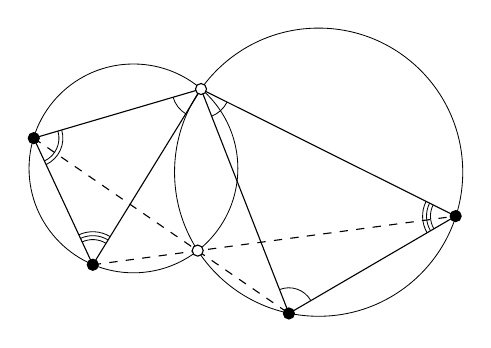
\begin{tikzpicture}[x=0.6cm,y=0.6cm]
			\draw [line width=0.3,shift={(-0.11,3.78)}] (-163.58:0.37cm) arc (-163.58:-121.62:0.37cm);
			\draw [line width=0.3,shift={(-0.11,3.78)}] (-68.6:0.37cm) arc (-68.6:-26.57:0.37cm);
			\draw [shift={(-3.65,2.74)}, line width=0.3] (-64.94:0.32cm) arc (-64.94:16.42:0.32cm);
			\draw [shift={(-3.65,2.74)}, line width=0.3] (-64.94:0.37cm) arc (-64.94:16.42:0.37cm);
			\draw [shift={(1.75,-0.96)},line width=0.3] (30.16:0.32cm) arc (30.16:111.40:0.32cm);
			\draw [shift={(-2.4,0.06)},line width=0.3] (58.38:0.32cm) arc (58.38:115.06:0.32cm);
			\draw [shift={(-2.4,0.06)},line width=0.3] (58.38:0.37cm) arc (58.38:115.06:0.37cm);
			\draw [shift={(-2.4,0.06)},line width=0.3] (58.38:0.42cm) arc (58.38:115.06:0.42cm);
			\draw [shift={(5.28,1.09)},line width=0.3] (153.43:0.32cm) arc (153.43:210.16:0.32cm);
			\draw [shift={(5.28,1.09)},line width=0.3] (153.43:0.37cm) arc (153.43:210.16:0.37cm);
			\draw [shift={(5.28,1.09)},line width=0.3] (153.43:0.42cm) arc (153.43:210.16:0.42cm);
			\draw [line width=0.3] (-1.54,2.1) circle (2.21);
			\draw [line width=0.3] (2.38,2.02) circle (3.05);
			\draw[dashed]  (-3.65,2.74)-- (1.75,-0.97);
			\draw[dashed]  (-2.4,0.06)-- (5.28,1.09);
			\draw (-3.65,2.74)-- (-2.4,0.06)-- (-0.11,3.78)-- cycle;
			\draw[fill=black, fill opacity=0] (-0.11,3.78)-- (1.75,-0.97)-- (5.28,1.09)-- cycle;
			\draw [fill=white] (-0.18,0.36) circle (2pt);
			\draw [fill=black] (-2.4,0.06) circle (2pt);
			\draw [fill=white] (-0.11,3.78) circle (2pt);
			\draw [fill=black] (-3.65,2.74) circle (2pt);
			\draw [fill=black] (1.75,-0.97) circle (2pt);
			\draw [fill=black] (5.28,1.09) circle (2pt);
		\end{tikzpicture} & & 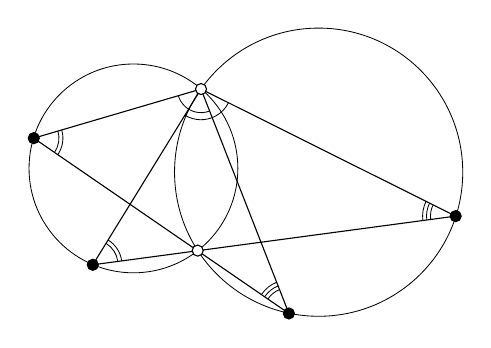
\begin{tikzpicture}[x=0.6cm,y=0.6cm]			
			\draw [shift={(-0.11,3.78)}, line width=0.3] (-163.58:0.30cm) arc (-163.58:-68.6:0.30cm);
			\draw [shift={(-0.11,3.78)},line width=0.3] (-121.62:0.39cm) arc (-121.62:-26.57:0.39cm);
			\draw [line width=0.3,shift={(5.28,1.09)}] (153.43:0.32cm) arc (153.43:187.59:0.32cm);
			\draw [line width=0.3,shift={(5.28,1.09)}] (153.43:0.37cm) arc (153.43:187.59:0.37cm);
			\draw [line width=0.3,shift={(5.28,1.09)}] (153.43:0.42cm) arc (153.43:187.59:0.42cm);
			\draw [line width=0.3,shift={(1.75,-0.96)}] (111.4:0.32cm) arc (111.4:145.56:0.32cm);
			\draw [line width=0.3,shift={(1.75,-0.96)}] (111.4:0.37cm) arc (111.4:145.56:0.37cm);
			\draw [line width=0.3,shift={(1.75,-0.96)}] (111.4:0.42cm) arc (111.4:145.56:0.42cm);
			\draw [shift={(-2.4,0.06)},line width=0.3] (7.59:0.32cm) arc (7.59:58.38:0.32cm);
			\draw [shift={(-3.65,2.74)},line width=0.3] (-34.44:0.32cm) arc (-34.44:16.42:0.32cm);
			\draw [shift={(-2.4,0.06)},line width=0.3] (7.59:0.37cm) arc (7.59:58.38:0.37cm);
			\draw [shift={(-3.65,2.74)},line width=0.3] (-34.44:0.37cm) arc (-34.44:16.42:0.37cm);
			\draw [line width=0.3] (-1.54,2.1) circle (2.21);
			\draw [line width=0.3] (2.38,2.02) circle (3.05);
			\draw[fill=black, fill opacity=0] (-3.65,2.74)-- (1.75,-0.97)-- (-0.11,3.78)-- cycle;
			\draw[fill=black, fill opacity=0] (-0.11,3.78)-- (-2.4,0.06)-- (5.28,1.09)-- cycle;
			\draw [fill=white] (-0.18,0.36) circle (2pt);
			\draw [fill=black] (-2.4,0.06) circle (2pt);
			\draw [fill=white] (-0.11,3.78) circle (2pt);
			\draw [fill=black] (-3.65,2.74) circle (2pt);
			\draw [fill=black] (1.75,-0.97) circle (2pt);
			\draw [fill=black] (5.28,1.09) circle (2pt);
		\end{tikzpicture} & 
	\end{tabularx}
\end{figure}

In jedem Fall solltet ihr euch folgende Strategie merken:
\begin{quote}\itshape
	Wenn sich in einer Aufgabe zwei Kreise schneiden, dann schaut euch die Drehstreckung um einen der beiden Schnittpunkte an, die den einen Kreis auf den anderen Kreis abbildet! Diese Drehstreckung kann auch als Projektion durch den anderen Schnittpunkt beschrieben werden.
\end{quote}

Wenn ihr diese Strategie verinnerlicht habt, dann könnt ihr euch die obigen Ähnlichkeiten immer wieder herleiten, ganz egal, ob ihr ein Auge für solche Konfigurationen habt oder nicht.

Bearbeitet an dieser Stelle die folgenden beiden Beispielaufgaben. Wie üblich findet ihr am Ende des Kapitels Tipps und am Ende des Heftes Lösungen zu diesen Aufgaben.

\begin{aufgabe*}\label{aufgabe:IMO2005_5}
	Sei $ABCD$ ein konvexes Viereck mit $\abs{BC}=\abs{DA}$. Auf den Seiten $\overline{BC}$ und~$\overline{DA}$ liegen Punkte $E$~und~$F$ mit $\abs{BE}=\abs{DF}$. Die Geraden $AC$ und~$BD$ schneiden sich in~$P$, die Geraden $AC$ und~$EF$ schneiden sich in~$Q$ und die Geraden $BD$ und~$EF$ schneiden sich in~$R$. Die Umkreise $\odot BCP$ und $\odot DAP$ schneiden sich neben in~\(P\) noch zusätzlich in~$S$.
	\begin{enumerate}
		\item \label{teilaufgabe:IMO2005_5a}Zeige, dass $BERS$, $CEQS$, $DFRS$ und $AFQS$ Sehnenvierecke sind.
		\item \label{teilaufgabe:IMO2005_5b}Zeige, dass $PQRS$ ein Sehnenviereck ist.
	\end{enumerate}
\end{aufgabe*}

\begin{aufgabe*}\label{aufgabe:FermatPunkt}
	Sei $ABC$ ein Dreieck. Auf die Seiten $\overline{BC}$, $\overline{CA}$ und~$\overline{AB}$ werden nach außen gleichseitige Dreiecke $BXC$, $CYA$ und $AZB$ aufgesetzt.
	\begin{enumerate}
		\item \label{teilaufgabe:FermatPunkt}Beweise, dass sich die Umkreise $\odot BXC$, $\odot CYA$ und $\odot AZB$ in einem Punkt~$P$ schneiden.
		\item \label{teilaufgabe:GeradenSchneidenSichImFermatPunkt}Beweise, dass die Geraden $AX$, $BY$ und~$CZ$ sich ebenfalls in~$P$ schneiden.
	\end{enumerate}
\end{aufgabe*}

\subsection*{Aufgesetzte Dreiecke}
Es gibt einen Typ von Aufgaben, in denen auf die Seiten eines Dreiecks weitere Dreiecke aufgesetzt werden; zu zeigen ist üblicherweise, dass das Dreieck, das von den Spitzen der aufgesetzten Dreiecke gebildet wird, eine bestimmte Eigenschaft hat. Beispiele für diesen Aufgabentyp sind Aufgabe~\ref{aufgabe:SatzVonAubel}, Aufgabe~\ref{aufgabe:SatzVonAubelAufSteroiden} und der Satz von Napoleon:
\begin{aufgabe*}\label{aufgabe:SatzVonAubel}
	Sei $ABC$ ein Dreieck. Auf die Seiten $\overline{CA}$ und~$\overline{AB}$ werden nach außen gleichschenklig-rechtwinklige Dreiecke $YCA$ mit Basis~$\overline{CA}$ und $ZAB$ mit Basis~$\overline{AB}$ aufgesetzt. Sei $M$ der Mittelpunkt von~$\overline{BC}$. Zeige, dass das Dreieck $MYZ$ gleichschenklig-rechtwinklig ist.
\end{aufgabe*}
\begin{aufgabe*}\label{aufgabe:SatzVonAubelAufSteroiden}
	Sei $ABC$ ein Dreieck. Auf die Seiten $\overline{BC}$, $\overline{CA}$ und~$\overline{AB}$ werden nach außen Dreiecke $BXC$, $CYA$ und $AZB$ aufgesetzt.
	% Tien: Ich habe bei der Aufzählung der Dreiecke das "und" entfernt, damit die "45°" nicht auf die nächste Zeile rutschen.
	Dabei gelte $\winkel XBC=\winkel BCX=15^\circ$, $\winkel YCA=\winkel ABZ=45^\circ$ und $\winkel CAY=\winkel ZAB=30^\circ$. Zeige, dass das Dreieck $XYZ$ gleichschenklig-rechtwinklig ist.
\end{aufgabe*}
\begin{satzmitnamen}[Satz von Napoleon]
	Sei $ABC$ ein Dreieck. Auf die Seiten $\overline{BC}$, $\overline{CA}$ und~$\overline{AB}$ werden nach außen gleichseitige Dreiecke $XBC$, $YCA$ und $ZAB$ aufgesetzt. Sei $A_1$ der Mittelpunkt von $XBC$, $B_1$~der Mittelpunkt von $YCA$ und $C_1$~der Mittelpunkt von $ZAB$. Dann ist $A_1B_1C_1$ ebenfalls ein gleichseitiges Dreieck.
\end{satzmitnamen}

Diese Aufgaben lassen sich allesamt mithilfe von Drehstreckungen lösen.\footnote{Aufgabe~\ref{aufgabe:SatzVonAubel} hat auch eine recht einfache Lösung mit kongruenten Dreiecken.} Allerdings sind diese Lösungen alles andere als offensichtlich. Am Ende dieses Kapitels findet ihr Tipps zu den Aufgaben und am Ende des Heftes könnt ihr die Lösungen nachlesen.


\subsection*{Streckungen und Kreise}
Eine Streckung mit Zentrum~$Z$ bildet jeden Punkt~$X$ auf einen Punkt~$X'$ ab, sodass $Z$,~$X$ und~$X'$ auf einer Geraden liegen. Aus dieser trivialen Beobachtung ergeben sich viele nicht-triviale Folgerungen, wovon wir euch einige in diesem Unterkapitel nahebringen wollen.

Wir beginnen mit dem Kreisberührungslemma, das euch schon als Übungsaufgabe zur Inversion am Kreis im Heft für Klasse~9 begegnet ist. Es wird euch also wenig überraschen, dass das Kreisberührungslemma auch einen sehr eleganten Beweis mit Inversion zulässt (und wenn ihr diese Aufgabe noch nicht bearbeitet habt, sei sie euch ausdrücklich ans Herz gelegt).

\begin{satzmitnamen}[Kreisberührungslemma]
	Sei $\Omega$ ein Kreis und $A$,~$B$ zwei Punkte auf~$\Omega$. Der Kreis~$\omega$ berühre $\Omega$ in~$P$ und die Gerade~$AB$ in~$Q$. Schließlich bezeichnen wir mit $S$~und~$N$ die Bogenmittelpunkte der beiden Bögen~$\wideparen{AB}$ von~$\Omega$, sodass $N$ auf der gleichen Seite von~$AB$ wie~$\omega$ liegt und $S$ auf der anderen Seite.
	\begin{enumerate}
		\item \label{itm:Kreisberuhrung}
		Wenn $\omega$ den Kreis~$\Omega$ von innen berührt, dann verläuft die Gerade~$PQ$ durch~$S$. Wenn sich die Kreise von außen berühren, verläuft $PQ$ durch~$N$.
		\item \label{itm:KreisberuhrungProdukt}
		Wenn $\omega$ den Kreis~$\Omega$ von innen berühren, gilt $\abs{SP}\cdot \abs{SQ}=\abs{SA}^2$. Wenn sich die Kreise von außen berühren, gilt $\abs{NP}\cdot \abs{NQ}=\abs{NA}^2$.
	\end{enumerate}
\end{satzmitnamen}

\begin{figure}[ht]
	\centering
	\begin{tabularx}{\textwidth}{X c X c X}
		& 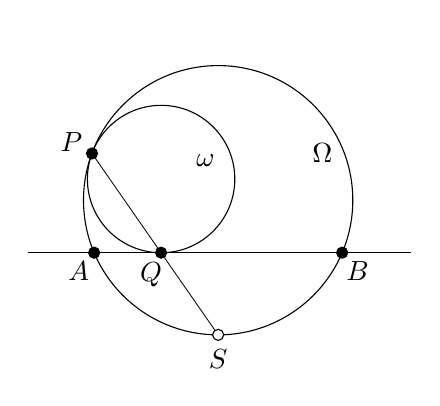
\begin{tikzpicture}[x=0.45cm,y=0.45cm]
			\draw  (2.56,0.38) circle (3.8);
			\draw [domain=-2.8:8] plot(\x,{(-17.86-0*\x)/16.24});
			\draw  (0.95,0.978) circle (2.08);
			\draw[line width=0.3]  (-1,1.7)-- (2.56,-3.42);
			\draw [fill=black] (-1,1.7) circle (2pt) node[shift={(150:2ex)}] {$P$};
			\draw [fill=white] (2.56,-3.42) circle (2pt) node[shift={(270:2ex)}] {$S$};
			\draw [fill=black] (0.95,-1.1) circle (2pt) node[shift={(245:2ex)}] {$Q$};
			\draw [fill=black] (-0.94,-1.1) circle (2pt) node[shift={(230:2ex)}] {$A$};
			\draw [fill=black] (6.06,-1.1) circle (2pt) node[shift={(310:2ex)}] {$B$};
			\node at (5.5, 1.7) {$\Omega$};
			\node at (2.2, 1.5) {$\omega$};
			\node[above] at (2.56,4.18) {\phantom{$N$}};
		\end{tikzpicture} & & 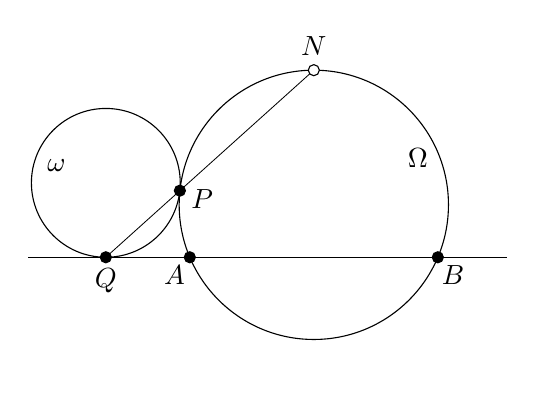
\begin{tikzpicture}[x=0.45cm,y=0.45cm]
			\draw  (2.56,0.38) circle (3.8);
			\draw [domain=-5.5:8] plot(\x,{(-17.864-0*\x)/16.24});
			\draw  (-3.31,1.00) circle (2.10);
			\draw[line width=0.3]  (-3.31,-1.1)-- (2.56,4.18);
			\draw [fill=black] (-1.22,0.78) circle (2pt) node[shift={(-20:2ex)}] {$P$};
			\draw [fill=black] (-0.94,-1.1) circle (2pt) node[shift={(230:2ex)}] {$A$};
			\draw [fill=black] (6.06,-1.1) circle (2pt) node[shift={(310:2ex)}] {$B$};
			\draw [fill=white] (2.56,4.18) circle (2pt) node[shift={(90:2ex)}] {$N$};
			\draw [fill=black] (-3.31,-1.1) circle (2pt) node[shift={(-90:2ex)}] {$Q$};
			\node at (5.5, 1.7) {$\Omega$};
			\node at (-4.7, 1.5) {$\omega$};
			\node[below] at (2.56,-3.42) {\phantom{$S$}};
		\end{tikzpicture} & 
	\end{tabularx}
\end{figure}

\begin{proof}
	Wir nehmen an, dass sich $\omega$~und~$\Omega$ von innen berühren; der andere Fall geht analog. Sei $\sigma$ die Streckung mit Zentrum~$P$, die $\omega$~auf~$\Omega$ abbildet. Dann ist $\sigma(AB)$ eine Tangente an~$\Omega$. Außerdem ist $\sigma(AB)$ parallel zu~$AB$. Es gibt aber nur zwei Tangenten an~$\Omega$, die parallel zu~$AB$ sind, nämlich die Tangenten in $S$~und~$N$. Es gilt also $\sigma(Q)=S$ oder $\sigma(Q)=N$. Weil $\omega$ den Kreis~$\Omega$ von innen berührt, muss $\sigma$ einen Streckfaktor
	% Tien: Ich habe mal $>1$ ausgeschrieben
	größer~$1$ haben. Also liegt $\sigma(Q)$ auf der Verlängerung von~$\overline{PQ}$ über~$Q$ hinaus. Also kommt nur $\sigma(Q)=S$ in Frage und wir erhalten, dass $S$ auf der Geraden~$PQ$ liegt. Damit ist Behauptung~\ref{itm:Kreisberuhrung} gezeigt.
	
	Die Behauptung~\ref{itm:KreisberuhrungProdukt} lässt sich mithilfe ähnlicher Dreiecke beweisen: Weil $S$ der Bogenmittelpunkt von~$\wideparen{AB}$ ist, muss das Dreieck $ABS$ gleichschenklig sein und es gilt $\winkel SAB=\winkel ABS$. Nach dem Peripheriewinkelsatz gilt $\winkel ABS=APS$. Es folgt also $\winkel SAQ=\winkel APS$. Weil die Dreiecke $ASQ$ und $ASP$ außerdem den Winkel $\winkel QSA=\winkel PSA$ gemeinsam haben, sind sie ähnlich. Es folgt $\abs{SA}/\abs{SQ}=\abs{SP}/\abs{SA}$ bzw.\ nach Umstellen $\abs{SP}\cdot\abs{SQ}=\abs{SA}^2$, wie behauptet.
\end{proof}

Im Kapitel zur Inversion aus dem Heft für Klasse~9 habt ihr gelernt, dass ihr, wann immer sich zwei Kreise berühren, am Berührpunkt (oder einem anderen Punkt auf einem der beiden Kreise) invertieren solltet. Dieser Strategie stellen wir nun eine weitere zur Seite:
\begin{quote}\itshape
	Wenn sich in einer Aufgabe zwei Kreise berühren, dann betrachtet die Streckung am Berührpunkt, die den einen Kreis auf den anderen abbildet!
\end{quote}
Auch wenn sich zwei Kreise nicht berühren, kann es sehr nützlich sein, den einen Kreis auf den anderen zu strecken. Auf diese Weise erhalten wir zum Beispiel einen sehr eleganten Beweis des folgenden Satzes:

\begin{satzmitnamen}[Satz von Monge]
	Seien $\omega_1$,~$\omega_2$ und~$\omega_3$ drei Kreise. Wir nehmen an, dass die Radien der Kreise paarweise verschieden sind und dass keiner der drei Kreise innerhalb eines der anderen beiden Kreise liegt. Die äußeren gemeinsamen Tangenten von $\omega_1$~und~$\omega_2$ schneiden sich in~$T_{1,2}$, die äußeren gemeinsamen Tangenten von $\omega_2$~und~$\omega_3$ schneiden sich in~$T_{2,3}$ und die äußeren gemeinsamen Tangenten von $\omega_3$~und~$\omega_1$ schneiden sich in~$T_{3,1}$. Dann sind $T_{1,2}$,~$T_{2,3}$ und~$T_{3,1}$ kollinear.
	
	Eine analoge Aussage gilt, wenn wir nur für $\omega_1$ und $\omega_2$ den Schnittpunkt der äußeren gemeinsamen Tangenten betrachten und für die anderen beiden Paare von Kreisen jeweils den Schnittpunkt der inneren gemeinsamen Tangenten \embrace{vorausgesetzt, die Kreise liegen so, dass die inneren gemeinsamen Tangenten existieren}.
\end{satzmitnamen}

\begin{figure}[ht]
	\centering
	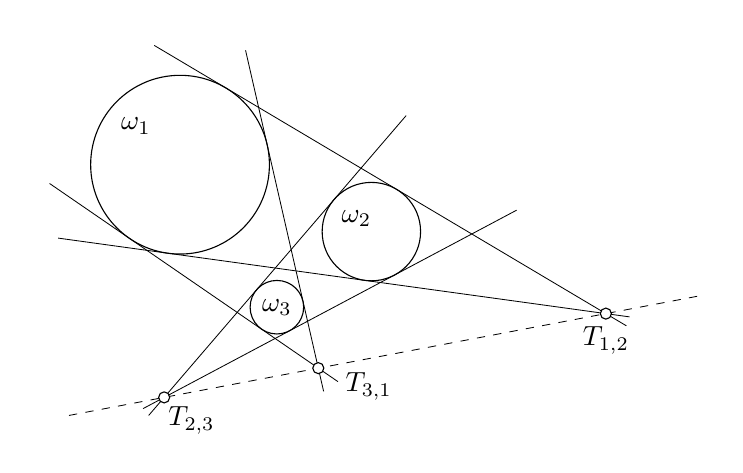
\begin{tikzpicture}[x=0.5cm,y=0.5cm]
		\clip (-5.35,-2.9) rectangle (12.1,7.7);
		\draw  (-1.48,4.22) circle (2.27);
		\draw  (3.38,2.52) circle (1.25);
		\draw  (0.98,0.6) circle (0.68);
		\coordinate (T12) at (9.336,0.437);
		\coordinate (T23) at (-1.883,-1.691);
		\coordinate (T31) at (2.032,-0.948);
		\draw [line width=0.3, shorten <=-3.5em,shorten >=-2ex] (-2.766,2.349) to (T31);
		\draw [line width=0.3, shorten <=-3.5em,shorten >=-2ex] (0.733,4.727) to (T31);
		\draw [line width=0.3, shorten <=-4em,shorten >=-2ex] (-1.79,1.971) to (T12);
		\draw [line width=0.3, shorten <=-3em,shorten >=-2ex] (-0.321,6.172) to (T12);
		\draw [line width=0.3, shorten <=-5em,shorten >=-2ex] (3.966,1.416) to (T23);
		\draw [line width=0.3, shorten <=-4em,shorten >=-2ex] (2.432,3.334) to (T23);
		\draw [dashed, line width=0.3,shorten <=-3.5em,shorten >=-3.4em] (T23) to (T12);
		\draw [fill=white] (T23) circle (2pt) node[shift={(320:3ex)}] {$T_{2,3}$};
		\draw [fill=white] (T31) circle (2pt) node[shift={(340:4.5ex)}] {$T_{3,1}$};
		\draw [fill=white] (T12) circle (2pt) node[shift={(270:2.25ex)}] {$T_{1,2}$};
		\node at (-2.6,5.2) {$\omega_1$};
		\node at (3,2.85) {$\omega_2$};
		\node at (0.98,0.6) {$\omega_3$};
	\end{tikzpicture}
\end{figure}

\begin{proof}
	Seien $r_1$,~$r_2$ und~$r_3$ die Radien von $\omega_1$,~$\omega_2$ und~$\omega_3$. Sei $\sigma_{1,2}$ die Streckung mit Zentrum~$T_{1,2}$ und Faktor $r_2/r_1$, die $\omega_1$~auf~$\omega_2$ abbildet. Analog sei $\sigma_{2,3}$ die Streckung mit Zentrum~$T_{2,3}$ und Faktor $r_3/r_2$, die $\omega_2$~auf~$\omega_3$ abbildet. Wir haben im vorherigen Unterkapitel gesehen, dass die Hintereinanderausführung $\sigma_{2,3}\circ \sigma_{1,2}$ wieder eine zentrische Streckung oder eine Verschiebung ist. Außerdem bildet $\sigma_{2,3}\circ \sigma_{1,2}$ den Kreis~$\omega_1$ auf den Kreis~$\omega_3$ ab. Nach Annahme haben $\omega_1$~und~$\omega_3$ verschiedene Radien, also kann $\sigma_{2,3}\circ \sigma_{1,2}$ keine Verschiebung sein. Es kommt also nur eine Streckung in Frage. Weil sich Streckfaktoren bei Hintereinanderausführung multiplizieren, hat $\sigma_{2,3}\circ \sigma_{1,2}$ den Streckfaktor $r_2/r_1\cdot r_3/r_2=r_3/r_1>0$. Es gibt aber nur eine Streckung mit positivem Streckfaktor, die $\omega_1$~auf~$\omega_3$ abbildet, nämlich die Streckung mit Zentrum~$T_{3,1}$ und Faktor $r_3/r_1$. Also muss $T_{3,1}$ das Zentrum von $\sigma_{2,3}\circ \sigma_{1,2}$ sein.
	
	Andererseits bilden sowohl~$\sigma_{1,2}$ als auch~$\sigma_{2,3}$ die Gerade $T_{1,2}T_{2,3}$ auf sich selbst ab. Also muss auch $\sigma_{2,3}\circ \sigma_{1,2}$ die Gerade $T_{1,2}T_{2,3}$ auf sich selbst abbilden. Dann muss aber das Streckzentrum von $\sigma_{2,3}\circ \sigma_{1,2}$ auf $T_{1,2}T_{2,3}$ liegen. Das ist genau die Aussage, die wir zeigen wollten.
	
	Die analoge Aussage folgt (wenig überraschend) analog, indem wir bemerken, dass es genau eine Streckung mit negativem Streckfaktor gibt, die $\omega_1$ auf $\omega_3$ abbildet, und dass das Zentrum dieser Streckung der Schnittpunkt der gemeinsamen inneren Tangenten von $\omega_1$ und $\omega_3$ ist.
\end{proof}

Merkt euch nicht (nur) die Aussage des Satzes von Monge, sondern merkt euch vor allem den Beweis! Der Satz von Monge wird häufig in Spezialfällen angewendet, die nicht sofort als solche zu erkennen sind (zum Beispiel, wenn in einer Aufgabe viele Inkreise vorkommen). Es wird euch leichter fallen, wenn ihr euch die konkreten Streckungen in einem Spezialfall anschaut (und damit den Satz von Monge für diesen Spezialfall erneut beweist).

\subsection*{Weitere Beispielaufgaben}
\begin{aufgabe*}\label{aufgabe:InAnkreis}
	Sei $ABC$ ein Dreieck. Der Inkreis~$\omega$ berühre die Strecke~$\overline{BC}$ in~$D$ und der Ankreis~$\omega_a$ gegenüber~$A$ berühre die Strecke~$\overline{BC}$ in~$E$. Sei $N$ der Punkt auf~$\omega$, der $D$ diametral gegenüber liegt, und sei $S$ der Punkt auf~$\omega_a$, der $E$ diametral gegenüber liegt. Zeige, dass $A$,~$D$ und~$S$ sowie $A$,~$E$ und~$N$ jeweils kollinear sind.
\end{aufgabe*}

\begin{figure}[ht]
	\centering
	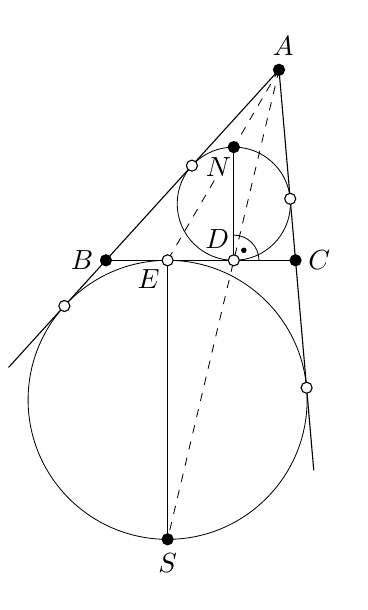
\begin{tikzpicture}[x=0.6cm,y=0.6cm]
		\draw [line width=0.3] (3.518,1.198) circle (1.198);
		\draw [line width=0.3] (2.117,-2.953) circle (2.953);
		\coordinate (A) at (4.475,4.032);
		\coordinate (B) at (0.811,0);
		\coordinate (C) at (4.825,0);
		\coordinate (D) at (3.518,0);
		\coordinate (E) at (2.117,0);
		\coordinate (N) at (3.518,2.396);
		\coordinate (S) at (2.117,-5.905);
		\coordinate (Tc) at (-0.068,-0.967);
		\coordinate (Tb) at (5.059,-2.697);
		\coordinate (Sc) at (2.632,2.004);
		\coordinate (Sb) at (4.712,1.302);
		\draw[shorten >=-3em] (A) to (Tc);
		\draw[shorten >=-3em] (A) to (Tb);
		\draw (B) to (C);
		\draw [dashed, line width=0.3] (A) to (S);
		\draw [dashed, line width=0.3] (A) to (N);
		\draw [dashed, line width=0.3, shorten <=1.4em] (N) to (E);
		\draw [line width=0.3] (N) to (D);
		\draw [line width=0.3] (E) to (S);
		\draw [line width=0.3, shift={(D)}] (0:0.32cm) arc (0:90:0.32cm);
		\fill [line width=0.3, shift={(D)}] (45:0.18cm) circle (1pt);
		\draw [fill=black] (A) circle (2pt) node[shift={(80:2ex)}] {$A$};
		\draw [fill=black] (B) circle (2pt) node[shift={(180:2ex)}] {$B$};
		\draw [fill=black] (C) circle (2pt) node[shift={(0:2ex)}] {$C$};
		\draw [fill=white] (D) circle (2pt) node[shift={(128:2.25ex)}] {$D$};
		\draw [fill=white] (E) circle (2pt) node[shift={(225:2.25ex)}] {$E$};
		\draw [fill=black] (N) circle (2pt) node[shift={(232:2.075ex)}] {$N$};
		\draw [fill=black] (S) circle (2pt) node[shift={(270:2ex)}] {$S$};
		\draw [fill=white] (Tc) circle (2pt);
		\draw [fill=white] (Tb) circle (2pt);
		\draw [fill=white] (Sc) circle (2pt);
		\draw [fill=white] (Sb) circle (2pt);
	\end{tikzpicture}
\end{figure}

\begin{aufgabe*}\label{aufgabe:551232}
	Gegeben ist ein Halbkreis~$\Omega$ mit Durchmesser~$\overline{AB}$. Auf~$\Omega$ liege ein Punkt~$C$, der von $A$~und~$B$ verschieden ist. Der Lotfußpunkt von~$C$ auf~$AB$ heiße~$D$. Ein Kreis $\omega$ liege außerhalb des Dreiecks $ADC$ und berühre gleichzeitig den Halbkreis~$\Omega$ sowie die Strecken $\overline{AB}$ und~$\overline{CD}$. Der Berührpunkt von~$\omega$ mit~$\overline{AB}$ sei~$E$. Zeige, dass die Strecken $\overline{AC}$ und~$\overline{AE}$ gleich lang sind. 
\end{aufgabe*}

(Diese Aufgabe habt ihr schon als Übungsaufgabe zur Inversion im Heft für Klasse~9 gesehen. Wenn ihr euch die Inversionslösung noch nicht überlegt habt, solltet ihr das nachholen.)

\begin{aufgabe*}\label{aufgabe:JuMaKlausur2014}
	Sei $ABCD$ ein konvexes Sehnenviereck mit Umkreis~$\Omega$ und Umkreismittelpunkt~$O$. Wir nehmen an, dass $\abs{AC}\neq \abs{BD}$. Die Diagonalen $AC$ und~$BD$ schneiden sich in~$E$. Eine Gerade~$\ell$ durch~$O$ schneide die Strecken $\overline{BE}$ und~$\overline{CE}$ in Punkten $P$~und~$Q$, sodass $\abs{EP}=\abs{EQ}$ gilt. Ein Kreis~$\omega$ berühre die Strecken $\overline{AE}$ und~$\overline{BE}$ und außerdem den Kreis~$\Omega$; sei $F$ der Berührpunkt mit~$\Omega$.
	% Tien: Ich habe das etwas umformuliert, damit der Berührpunkt eindeutig ist.
	Die Geraden $EF$ und~$\ell$ schneiden sich in~$M$. Beweise, dass die durch~$M$ gezogene Parallele zu~$AC$ den Kreis~$\Omega$ berührt.
\end{aufgabe*}


\newpage\phantom{newpage}\vfill\hrule\vspace{-1em}
\subsection*{Tipps zu den Beispielaufgaben}

\textbf{Tipps zu Aufgabe~\ref{aufgabe:IMO2005_5}.} Um~\ref{teilaufgabe:IMO2005_5a} zu zeigen, betrachte die Drehstreckung~$\sigma$ mit Zentrum~$S$, die den Umkreis $\odot BCP$ auf den Umkreis $\odot DAP$ abbildet. Was kannst du über $\sigma$ aussagen? Wiederhole dann das gleiche Argument mit $\overline{BE}$ und $\overline{DF}$ statt $\overline{BC}$ und $\overline{DA}$.

Für~\ref{teilaufgabe:IMO2005_5b} benutze~\ref{teilaufgabe:IMO2005_5a} und eine Winkeljagd.

\textbf{Tipps zu Aufgabe~\ref{aufgabe:FermatPunkt}.} Für~\ref{teilaufgabe:FermatPunkt} benutze eine Winkeljagd.

Um in~\ref{teilaufgabe:GeradenSchneidenSichImFermatPunkt} zu zeigen, dass sich $BY$ und $CZ$ in~$P$ schneiden, betrachte eine geeignete Drehstreckung mit Zentrum~$A$.

\textbf{Tipp zu Aufgabe~\ref{aufgabe:SatzVonAubel}.} Betrachte die Drehstreckung~$\sigma$ mit Zentrum~$Z$, Drehwinkel~$45^\circ$ und Faktor~$\sqrt{2}$. Welchen Punkt bildet $\sigma$ auf~$A$ ab? Zeige dann, dass $\sigma(M)=Y$.

\textbf{Tipp zu Aufgabe~\ref{aufgabe:SatzVonAubelAufSteroiden}.} Betrachte die Drehstreckung~$\sigma$ mit Zentrum~$Z$, Drehwinkel~$45^\circ$ und Faktor~$\sqrt{2}$. Welchen Punkt bildet $\sigma$ auf~$A$ ab? Zeige dann, dass $\sigma(X)=Y$.

\textbf{Tipp zu Aufgabe~\ref{aufgabe:InAnkreis}.} Betrachte die Streckung mit Zentrum~$A$, die den Inkreis~$\omega$ auf den Ankreis~$\omega_a$ schickt.

\textbf{Tipp zu Aufgabe~\ref{aufgabe:551232}.} Benutze das Kreisberührungslemma.

\textbf{Tipps zu Aufgabe~\ref{aufgabe:JuMaKlausur2014}.} Wie muss~$\ell$ liegen, damit die Bedingung $\abs*{EP}=\abs*{EQ}$ erfüllt ist?

Betrachte die Strecknung mit Zentrum~$F$, die~$\omega$ auf~$\Omega$ abbildet. Untersuche, worauf $\sigma$ den Punkt~$E$ und die Gerade~$AC$ abbildet.